\documentclass{beamer}
\usepackage[T1]{fontenc} % Use T1 Font Encoding
\usepackage{lmodern}     % Use Latin Modern Fonts as a more complete replacement
\usepackage{amsmath}     % Enhanced support for mathematical formulas
\usepackage{amsfonts,amsmath,oldgerm}
\usepackage{listings}
\usepackage{minted}
\usetheme{sintef}

\newcommand{\testcolor}[1]{\colorbox{#1}{\textcolor{#1}{test}}~\texttt{#1}}

\usefonttheme[onlymath]{serif}

\titlebackground*{assets/background}

\newcommand{\hrefcol}[2]{\textcolor{cyan}{\href{#1}{#2}}}

\title{Presentation du Projet Metier}
\subtitle{Mise en oeuvre et stabilisation d'un bras de drone quadrirotor}
\author{Encadre par:\hspace*{.3cm}Mr. TALEB\\Jury:\hspace*{.3cm}Mr. TALEB\hspace*{.3cm}Mr.SAADI\hspace*{.3cm}Mr. LAGRIOUI}
\course{Ahmed Amine NOUABI\\
		Mamane Bello Abdoul Hakim
}


\date{1st July 2024}

\begin{document}
\maketitle

% \begin{frame}

% This template is a based on \hrefcol{https://www.overleaf.com/latex/templates/sintef-presentation/jhbhdffczpnx}{SINTEF Presentation} from \hrefcol{mailto:federico.zenith@sintef.no}{Federico Zenith} and its derivation \hrefcol{https://github.com/TOB-KNPOB/Beamer-LaTeX-Themes}{Beamer-LaTeX-Themes} from Liu Qilong and Andrea Gasparini

% \vspace{\baselineskip}

% In the following you find a brief introduction on how to use \LaTeX\ and the beamer package to prepare slides, based on the one written by \hrefcol{mailto:federico.zenith@sintef.no}{Federico Zenith} for \hrefcol{https://www.overleaf.com/latex/templates/sintef-presentation/jhbhdffczpnx}{SINTEF Presentation}

% % This template is released under \hrefcol{https://creativecommons.org/licenses/by-nc/4.0/legalcode}{Creative Commons CC BY 4.0} license

% \end{frame}

\section{Introduction}

\begin{frame}{Objectifs du projet.}
	\begin{itemize}
		\item Stabiliser un bras rotative.
		\item Utilisation d'un capteur MPU6050 et un algorithme de calcul d'angle.
		\item Mise en oeuvre d'un controleur PID pour commander les moteurs.
	\end{itemize}
	\end{frame}

\begin{sidepic}{assets/pres-proj.png}{Presentation du projet.}
	Le projet consiste en la conception et la mise en œuvre d'un système de stabilisation pour une barre rotative à un degré de liberté. En utilisant un microcontrôleur Arduino et un capteur IMU MPU6050, nous avons développé un algorithme de contrôle PID pour maintenir la barre stable malgré les perturbations externes.
\end{sidepic}

\begin{frame}{Fonctionnement du systeme.}
	\begin{figure}
		\centering
		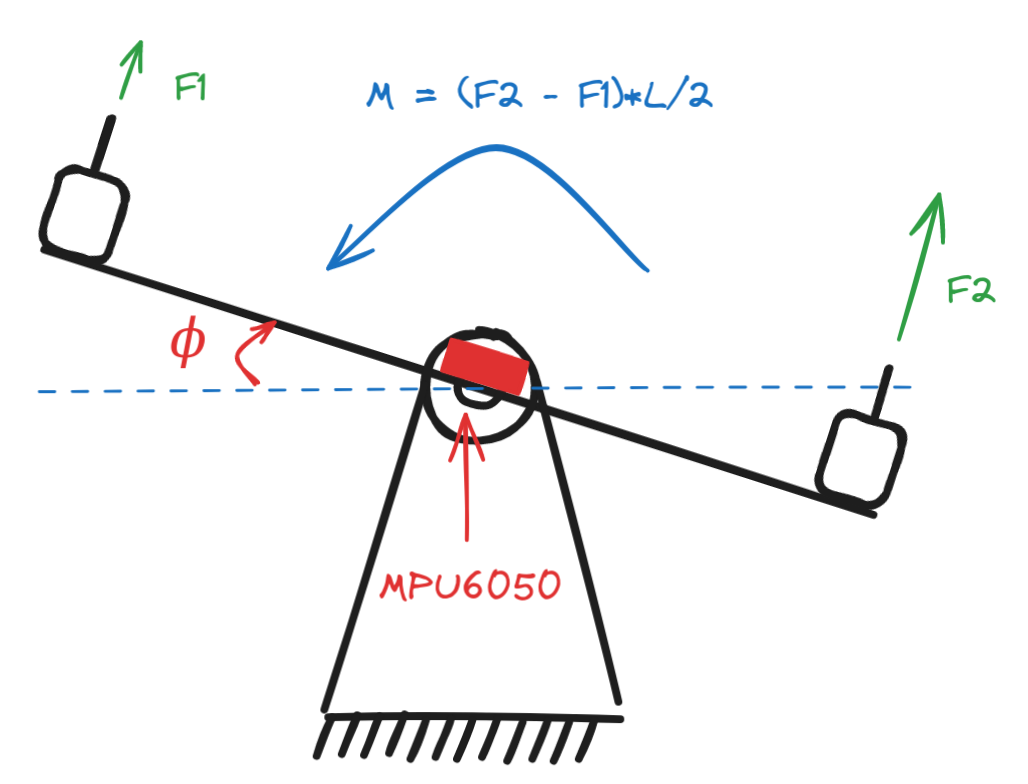
\includegraphics[width=0.4\textwidth]{assets/fonction.png}
		\caption{Fonctionnement du systeme.}
	\end{figure}
\end{frame}

\section{Conception du systeme}

\begin{frame}{Conception mecanique.}
\begin{figure}
	\centering
	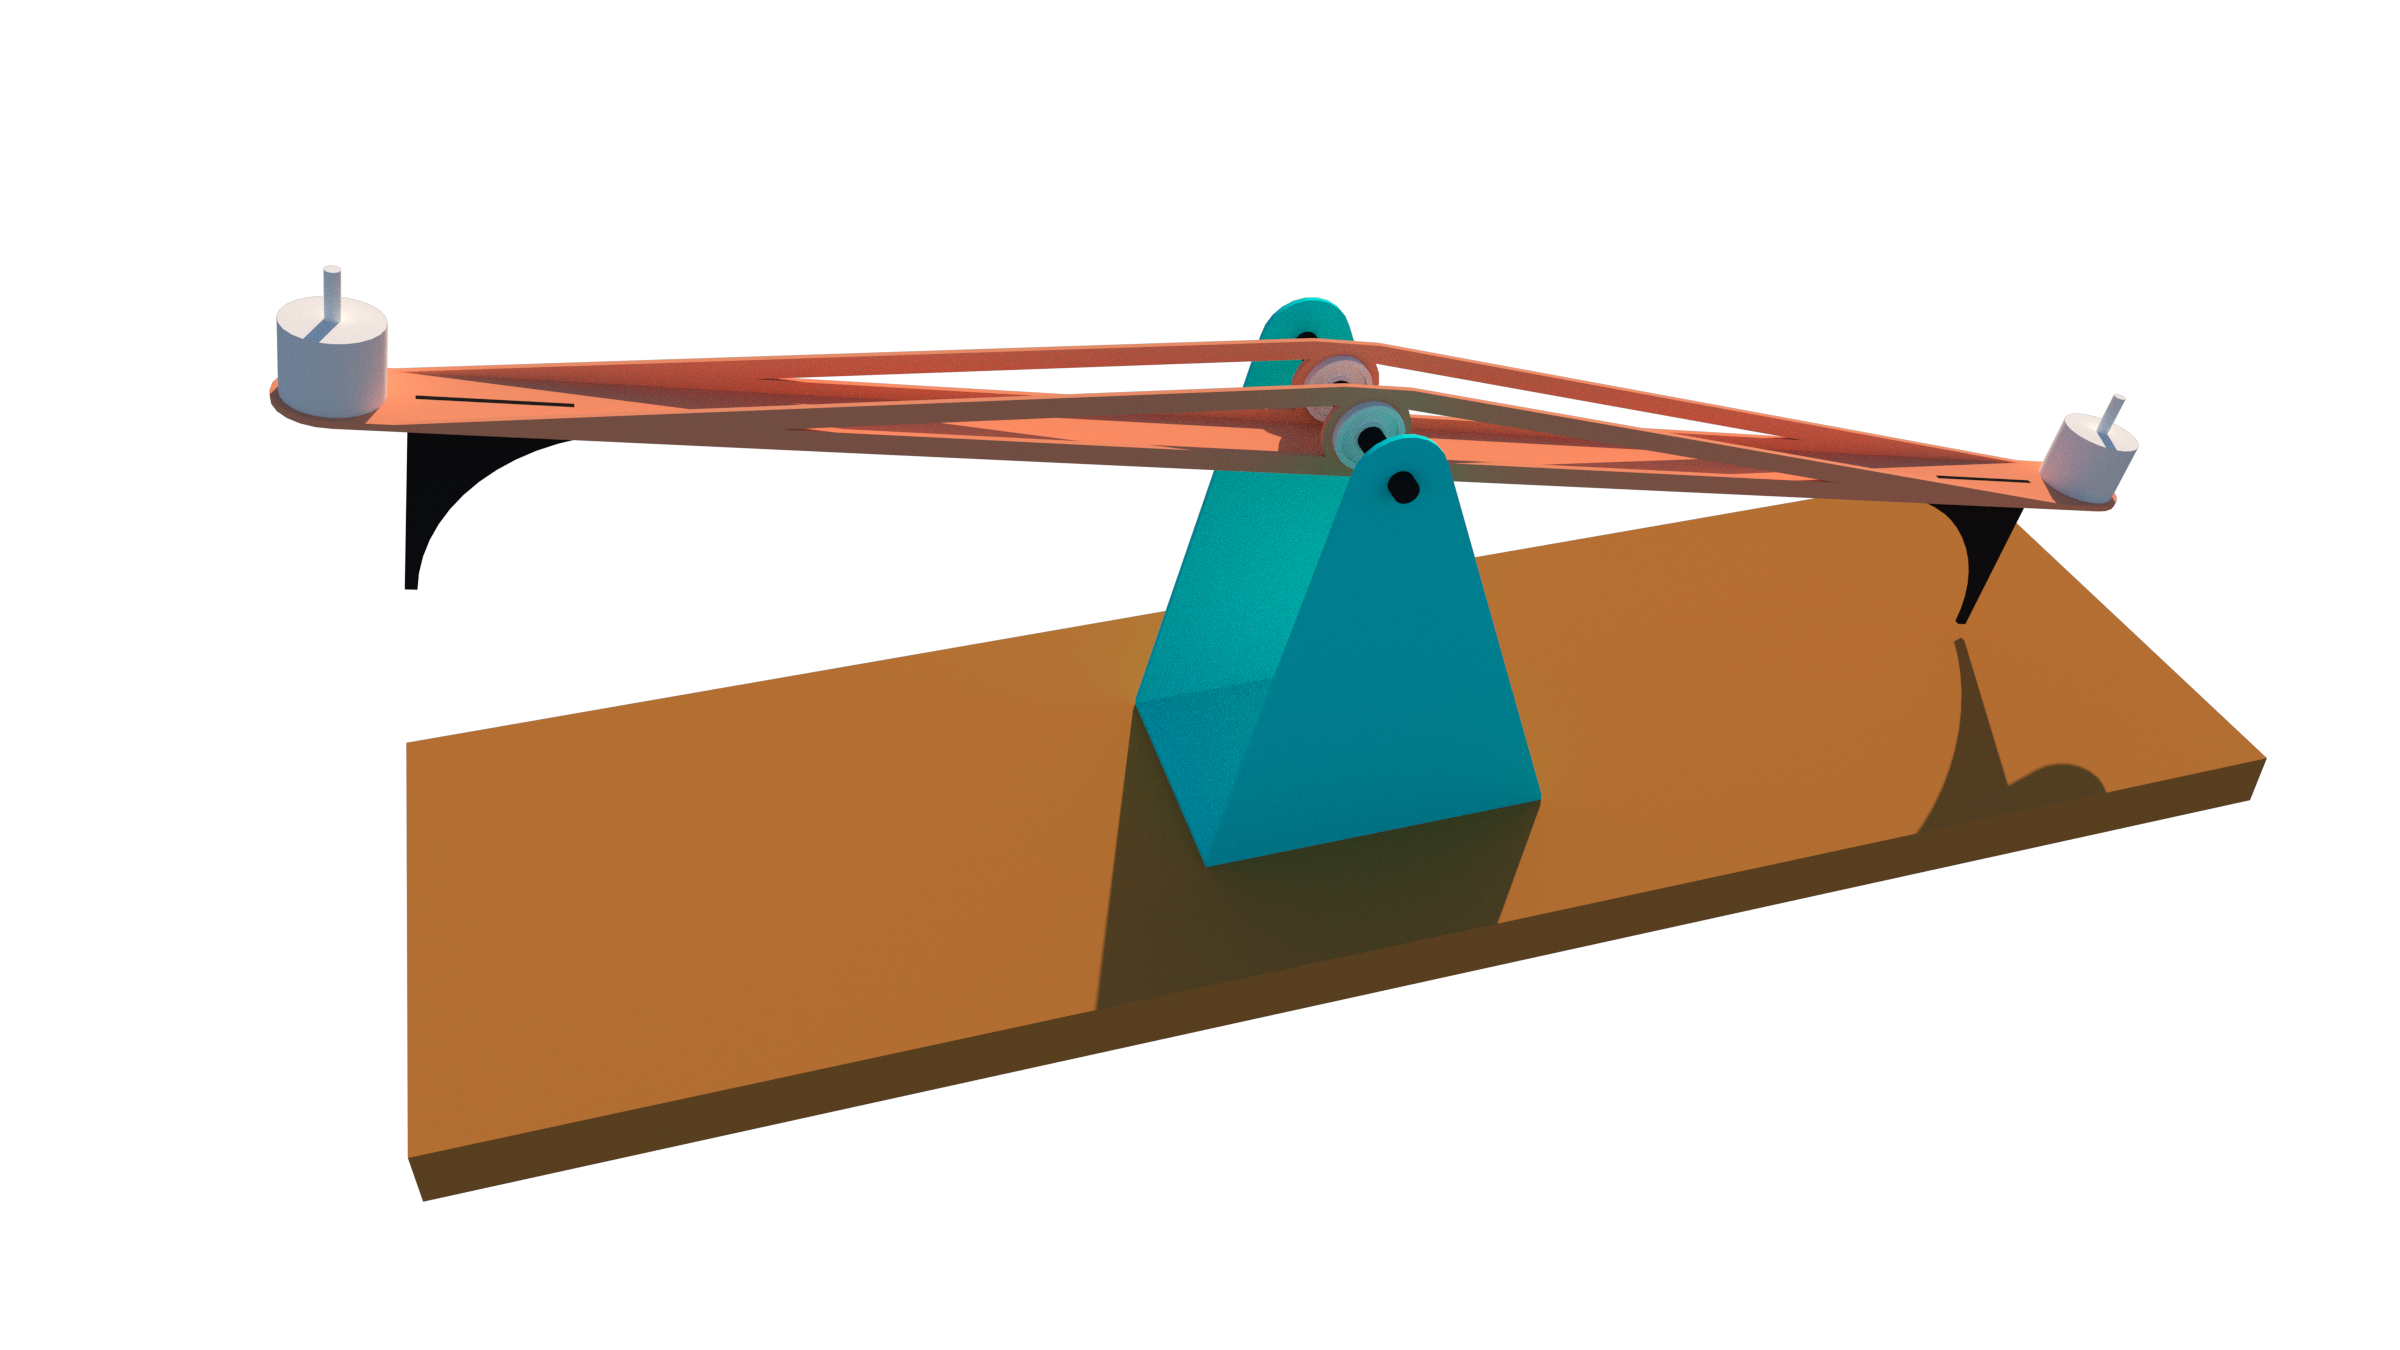
\includegraphics[width=0.6\textwidth]{assets/3d-cad.png}
	\caption{Modele mecanique 3D.}
\end{figure}
\end{frame}


\begin{sidepic}{assets/mpu6050.png}{Calcul d'angle}
	\begin{itemize}
		\item Le MPU6050 est un capteur qui combine un accéléromètre et un gyroscope.
		\item L'accéléromètre mesure l'accélération linéaire tandis que le gyroscope mesure la vitesse angulaire.
	\end{itemize}
\end{sidepic}

\begin{frame}[fragile]{Calcul d'angle par gyroscope}
	\begin{block}{Modele mathematique du gyroscope}
		\begin{equation*}
			\omega = \frac{d\phi}{dt}
		\end{equation*}
	\end{block}
\end{frame}

\begin{frame}[fragile]{Calcul d'angle par gyroscope}
	\begin{block}{Modele mathematique du gyroscope}
		\begin{equation*}
			\omega = \frac{d\phi}{dt}
		\end{equation*}
	\end{block}
	\begin{block}{Calcul d'angle par gyroscope}
		\begin{equation*}
			\hat{\phi}_{gyro}(n) =  \sum_{i=0}^{n} \omega(i) * T
		\end{equation*}
	\end{block}
	\begin{itemize}
		\item $T$ est le temps d'echantillonnage $0.004s$.  ($f_e = 250Hz$)
	\end{itemize}
\end{frame}

\begin{sidepic}{assets/drift.png}{Limitation du modele}
	\begin{itemize}
		\item Le gyroscope est sujet à des dérives.
		\item L'angle calculé par le gyroscope diverge avec le temps.
	\end{itemize}
	\begin{block}{Modele proche de la realite}
		\begin{equation*}
			\omega = \frac{d\phi}{dt} + b_g(t) + n_g(t)
		\end{equation*}
	\end{block}
	\begin{itemize}
		\item $b_g(t)$ est l'offset du gyroscope.
		\item $n_g(t)$ est le bruit du gyroscope.
	\end{itemize}
\end{sidepic}



\begin{frame}[fragile]{Calcul d'angle par accéléromètre}
	\begin{block}{Modele mathematique de l'accéléromètre}
		\begin{equation*}
			\vec{a} = -R * \vec{g}
		\end{equation*}
	\end{block}
	\begin{block}{Calcul d'angle par accéléromètre}
		\begin{align*}
			a_x &= g \sin(\phi) \\
			a_y &= -g \sin(\theta) \cos(\phi)\\
			a_z &= -g \cos(\theta) \cos(\phi)
		\end{align*}
		\begin{equation*}
			\hat{\phi}_{accelo}(n) = \arcsin\left(\frac{a_x(n)}{g}\right)
		\end{equation*}
	\end{block}
\end{frame}

\begin{frame}{Fusion des resultats}
	\begin{itemize}
		\item Pour pallier les dérives du gyroscope, on combine les résultats de l'accéléromètre et du gyroscope.
		\item En prenant $\alpha$ tres proche de 1, on donne plus de poids au gyroscope. ($\alpha = 0.9996$)
	\end{itemize}
	\begin{block}{Fusion des resultats}
		\begin{equation*}
			\hat{\phi}(n) = \alpha * \hat{\phi}_{gyro}(n) + (1 - \alpha) * \hat{\phi}_{accelo}(n)
		\end{equation*}
	\end{block}
\end{frame}


\begin{frame}{Commade des moteurs}
	\begin{itemize}
		\item on utilise un ESC (Electronic Speed Controller) pour commander le moteur.
		\item ESC est commandé par un signal PWM (Pulse Width Modulation).
	\end{itemize}
	\begin{block}{Plage de commande}
		\begin{equation*}
				1000\mu s \leq T_{on} \leq 2000\mu s
		\end{equation*}
	\end{block}
\end{frame}

\begin{frame}{Controleur PID}
	\begin{block}{Equation du controleur PID}
		\begin{equation*}
			u(t) = K_p * e(t) + K_i * \int e(t) dt + K_d * \frac{de(t)}{dt}
		\end{equation*}
	\end{block}
	\begin{itemize}
		\item Pour utiliser une comande symetrique. $\gamma = 1500 \pm u(t)$
		\item $\gamma$ valeur de la commande PWM du moteur.
		\item On limite $u(t)$ entre $-400$ et $400$.
	\end{itemize}
\end{frame}

\begin{frame}{Schema de controle}
	\begin{figure}
		\centering
		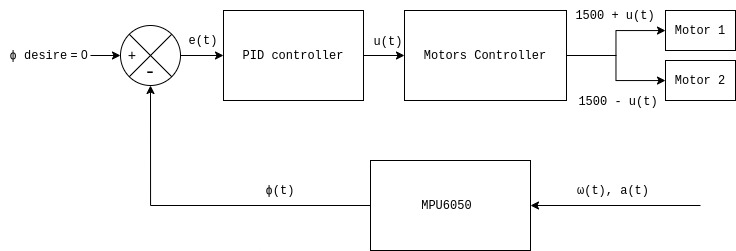
\includegraphics[width=0.9\textwidth]{assets/control.jpg}
		\caption{Schema de controle.}
	\end{figure}
\end{frame}

\begin{frame}{Montage Electrique}
	\begin{figure}
		\centering
		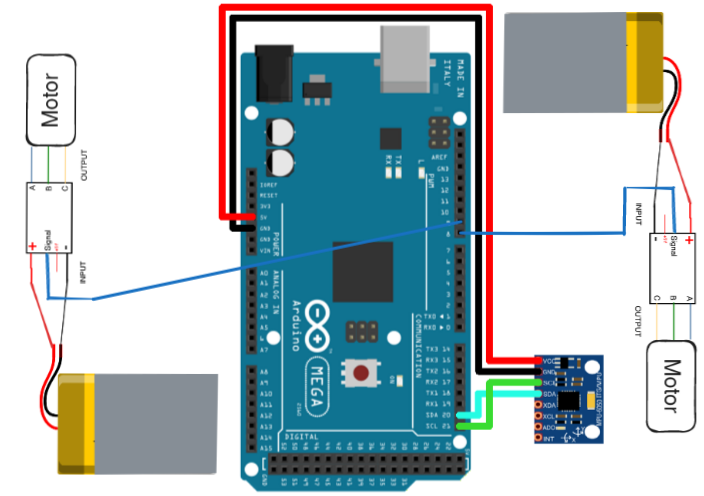
\includegraphics[width=0.5\textwidth]{assets/final-circuit.png}
		\caption{Montage Electrique.}
	\end{figure}
\end{frame}

\section{Conception Logiciel}

\begin{frame}{Conception Logiciel}
	\begin{itemize}
		\item Pour faciliter la maintenance et l'evolution du code, on a utilisé une approche orientée objet (OOP).
		\item On utilise la librairie \texttt{Wire} pour la communication I2C avec le capteur MPU6050.
		\item On utilise la librairie \texttt{ESC} pour la commande PWM des moteurs.
	\end{itemize}
\end{frame}

\begin{frame}{Composants Logiciel OOP}
	\begin{figure}
		\centering
		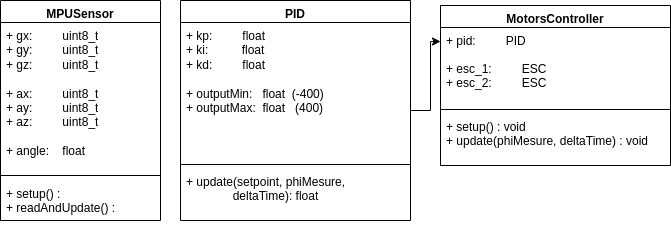
\includegraphics[width=0.9\textwidth]{assets/uml.jpg}
		\caption{UML des Composants Logiciel.}
	\end{figure}
\end{frame}


\begin{frame}[fragile]{Code Arduino - Setup}
	\begin{minted}{c}
	MPUSensor mpu;
	MotorsController motors;

	double deltaTime_micros = 0.004 / 1000000.0;

	void setup() {
		mpu.setup();
		motors.setup();
	}
	\end{minted}
\end{frame}

\begin{frame}[fragile]{Code Arduino - Loop}
	\begin{minted}{c}
	void loop() {
		current_micros = micros();

		mpu.readAndUpdate();
		motors.update(mpu.angle, deltaTime);

		// Pour assurer une boucle de controle de 4ms.
		while (micros() - current_micros < deltaTime_micros);
	}
	\end{minted}
\end{frame}

\section{Conclusion}

\begin{frame}{Conclusion}
	\begin{itemize}
		\item En partant d'ici on peut envisager l'implementation ou de creer un environement de simulation pour tester le systeme.
		\item On peut aussi considerer a ajouter differentes strategies de controle et d'acquisition pour un benchmark de resultats.
	\end{itemize}
\end{frame}

% \begin{frame}[fragile]{Title page}
% To set a typical title page, you call some commands in the preamble:
% \begin{block}{The Commands for the Title Page}
% \begin{verbatim}
% \title{Sample Title}
% \subtitle{Sample subtitle}
% \author{First Author, Second Author}
% \date{\today} % Can also be (ab)used for conference name &c.
% \end{verbatim}
% \end{block}
% You can then write out the title page with \verb|\maketitle|.

% To set a \textbf{background image} use the \verb|\titlebackground| command 
% before \verb|\maketitle|; its only argument is the name (or path) of a graphic 
% file.

% If you use the \textbf{starred version} \verb|\titlebackground*|, the image 
% will be clipped to a split view on the right side of the title slide.

% \end{frame}

% \begin{frame}[fragile]{Writing a Simple Slide}
% \framesubtitle{It's really easy!}
% \begin{itemize}[<+->]
% \item A typical slide has bulleted lists
% \item These can be uncovered in sequence
% \end{itemize}
% \begin{block}{Code for a Page with an Itemised List}<+->
% \begin{verbatim}
% \begin{frame}{Writing a Simple Slide}
%   \framesubtitle{It's really easy!}
%   \begin{itemize}[<+->]
%     \item A typical slide has bulleted lists
%     \item These can be uncovered in sequence
%   \end{itemize}\end{frame}
% \end{verbatim}
% \end{block}
% \end{frame}

% \section{Personalization}

% \footlinecolor{sintefyellow}
% \begin{frame}[fragile]{Changing Slide Style}
% \begin{itemize}
% \item You can select the white or \textit{maincolor} \textbf{slide style} \emph{in the 
% preamble} with \verb|\themecolor{white}| (default) or \verb|\themecolor{main}|
%       \begin{itemize}
%       \item You should \emph{not} change these within the document: Beamer does 
%       not like it
%       \item If you \emph{really} must, you may have to add 
%       \verb|\usebeamercolor[fg]{normal text}| in the slide
%       \end{itemize}
% \item You can change the \textbf{footline colour} with 
% \verb|\footlinecolor{color}|
%       \begin{itemize}
%       \item Place the command \emph{before} a new \verb|frame|
%       \item There are four ``official'' colors: 
%       \testcolor{maincolor}, \testcolor{sintefyellow}, 
%       \testcolor{sintefgreen}, \testcolor{sintefdarkgreen}
%       \item Default is no footline; you can restore it with 
%       \verb|\footlinecolor{}|
%       \item Others may work, but no guarantees!
%       \item Should \emph{not} be used with the \verb|maincolor| theme!
%       \end{itemize}
% \end{itemize}
% \end{frame}

% \begin{frame}[fragile]{Blocks}
% \begin{columns}
% \begin{column}{0.3\textwidth}
% \begin{block}{Standard Blocks}
% These have a color coordinated with the footline (and grey in the blue theme)
% \begin{verbatim}
% \begin{block}{title}
% content...
% \end{block}
% \end{verbatim}
% \end{block}
% \end{column}
% \begin{column}{0.7\textwidth}
% \begin{colorblock}[black]{sinteflightgreen}{Colour Blocks}
% Similar to the ones on the left, but you pick the colour. Text will be white by 
% default, but you may set it with an optional argument.
% \small
% \begin{verbatim}
% \begin{colorblock}[black]{sinteflightgreen}{title}
% content...
% \end{colorblock}
% \end{verbatim}
% \end{colorblock}
% The ``official'' colours of colour blocks are: \testcolor{sinteflilla}, 
% \testcolor{maincolor}, \testcolor{sintefdarkgreen}, and 
% \testcolor{sintefyellow}.
% \end{column}
% \end{columns}
% \end{frame}

% \footlinecolor{}
% \begin{frame}[fragile]{Using Colours}
% \begin{itemize}[<alert@2>]
%   \item You can use colours with the
%         \verb|\textcolor{<color name>}{text}| command
%   \item The colours are defined in the \texttt{sintefcolor} package:
%   \begin{itemize}
%   \item Primary colours: \testcolor{maincolor} and its sidekick 
%   \testcolor{sintefgrey}
%   \item Three shades of green: \testcolor{sinteflightgreen}, 
%   \testcolor{sintefgreen}, \testcolor{sintefdarkgreen}
%   \item Additional colours: \testcolor{sintefyellow}, \testcolor{sintefred}, 
%         \testcolor{sinteflilla}
%         \begin{itemize}
%         \item These may be shaded---see the \verb|sintefcolor| documentation or 
%         the \hrefcol{https://sintef.sharepoint.com/sites/stottetjenester/%
%         kommunikasjon/grafisk-profil-new/Sider/default.aspx}{SINTEF profile 
%         manual}
%         \end{itemize}
%   \end{itemize}
%   \item Do \emph{not} abuse colours: \verb|\emph{}| is usually enough
%   \item Use \verb|\alert{}| to bring the \alert<2->{focus} somewhere
%   \item<2- | alert@2> If you highlight too much, you don't highlight at all!
% \end{itemize}
% \end{frame}

% \begin{frame}[fragile]{Adding images}
% \begin{columns}
% \begin{column}{0.7\textwidth}
% Adding images works like in normal \LaTeX:
% \begin{block}{Code for Adding Images}
% \begin{verbatim}
% \usepackage{graphicx}
% % ...
% \includegraphics[width=\textwidth]
% {assets/logo_RGB}
% \end{verbatim}
% \end{block}
% \end{column}
% \begin{column}{0.3\textwidth}
% \includegraphics[width=\textwidth]
% {assets/logo_RGB}
% \end{column}
% \end{columns}
% \end{frame}

% \begin{frame}[fragile]{Splitting in Columns}
% Splitting the page is easy and common;
% typically, one side has a picture and the other text:
% \begin{columns}
% \begin{column}{0.6\textwidth}
% This is the first column
% \end{column}
% \begin{column}{0.3\textwidth}
% And this the second
% \end{column}
% \end{columns}
% \begin{block}{Column Code}
% \begin{verbatim}
% \begin{columns}
%     \begin{column}{0.6\textwidth}
%         This is the first column
%     \end{column}
%     \begin{column}{0.3\textwidth}
%         And this the second
%     \end{column}
%     % There could be more!
% \end{columns}
% \end{verbatim}
% \end{block}
% \end{frame}

% \begin{chapter}[assets/background_negative]{}{Special Slides}
% \begin{itemize}
% \item Chapter slides
% \item Side-picture slides
% \end{itemize}
% \end{chapter}

% \footlinecolor{sintefred}
% \begin{frame}[fragile]{Chapter slides}
% \begin{itemize}
% \item Similar to \verb|frame|s, but with a few more options
% \item Opened with \verb|\begin{chapter}[<image>]{<color>}{<title>}|
% \item Image is optional, colour and title are mandatory
% \item There are seven ``official'' colours: \testcolor{maincolor}, 
% \testcolor{sintefdarkgreen}, \testcolor{sintefgreen}, 
% \testcolor{sinteflightgreen}, \testcolor{sintefred}, \testcolor{sintefyellow}, 
% \testcolor{sinteflilla}.
%       \begin{itemize}
%       \item Strangely enough, these are \emph{more} than the official colours 
%       for the footline.
%       \item It may still be a nice touch to change the footline of following 
%       slides to the same color of a chapter slide. Your choice.
%       \end{itemize}
% \item Otherwise, \verb|chapter| behaves just like \verb|frame|.
% \end{itemize}
% \end{frame}

% \begin{sidepic}{assets/background_alternative}{Side-Picture Slides}
% \begin{itemize}
% \item Opened with \texttt{$\backslash$begin\{sidepic\}\{<image>\}\{<title>\}}
% \item Otherwise, \texttt{sidepic} works just like \texttt{frame}
% \end{itemize}
% \end{sidepic}

% \footlinecolor{}
% \begin{frame}
% \frametitle{Fonts}
% \begin{itemize}
% \item The paramount task of fonts is being readable
% \item There are good ones...
%   \begin{itemize}
%   \item {\textrm{Use serif fonts only with high-definition projectors}}
%   \item {\textsf{Use sans-serif fonts otherwise (or if you simply prefer 
% them)}}
%   \end{itemize}
% \item ... and not so good ones:
%   \begin{itemize}
%   \item {\texttt{Never use monospace for normal text}}
%   \item {\frakfamily Gothic, calligraphic or weird fonts: should always: be
%   avoided}
% \end{itemize}
% \end{itemize}
% \end{frame}

% \begin{frame}[fragile]{Look}
% \begin{itemize}
% \item To insert a final slide with the title and final thanks, use \verb|\backmatter|.
%       \begin{itemize}
%       \item The title also appears in footlines along with the author name, you can change this text with \verb|\footlinepayoff|
%       \item You can remove the title from the final slide with \verb|\backmatter[notitle]|
%       \end{itemize}
% \item The aspect ratio defaults to 16:9, and you should not change it to 4:3
%       for old projectors as it is inherently impossible to perfectly convert a 
%       16:9 presentation to 4:3 one; spacings \emph{will} break
%       \begin{itemize}
%       \item The \texttt{aspectratio} argument to the \texttt{beamer} class is
%             overridden by the SINTEF theme
%       \item If you \emph{really} know what you are doing, check the package
%             code and look for the \texttt{geometry} class.
%       \end{itemize}
% \end{itemize}
% \end{frame}

% \section{Summary}

% \begin{frame}
% \frametitle{Good Luck!}
% \begin{itemize}
% \item Enough for an introduction! You should know enough by now
% \item If you have any suggestions or corrections, feel free to contribute on the \hrefcol{https://github.com/pintorem/unicagliari-beamer-template}{GitHub repository}!
% You can \hrefcol{https://github.com/pintorem/unicagliari-beamer-template/issues/new}{open an issue} or \hrefcol{https://github.com/pintorem/unicagliari-beamer-template/fork}{fork the project} and directly propose your changes with a Pull Request. 
% \end{itemize}
% \end{frame}

\backmatter
\end{document}
